\documentclass[crop, tikz]{standalone}
\begin{document}
	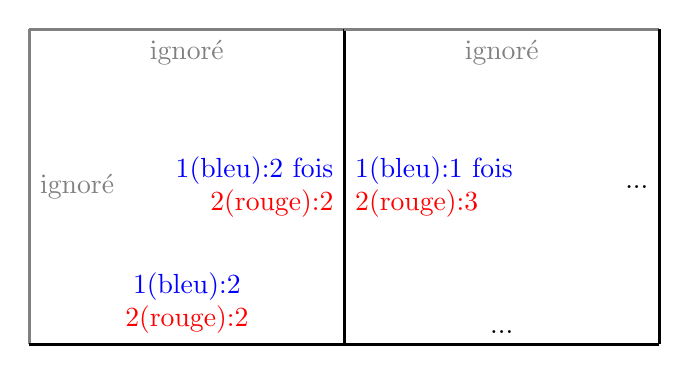
\begin{tikzpicture}
		\begin{scope}
			\coordinate (A1) at (0, 0);
			\coordinate (A2) at (0, 4);
			\coordinate (A3) at (4, 4);
			\coordinate (A4) at (4, 0);
			
			\draw [very thick, auto=right, color= gray] 
			(A1) -- node {ignor\'{e}} (A2) ;
			\draw [very thick, auto=right, color= gray] (A2) -- node {ignor\'{e}} (A3) ;
			\draw [very thick, auto=right] (A3)	-- node[align=right] {\textcolor{blue}{1(bleu):2 fois} \\ \textcolor{red}{2(rouge):2}} (A4); 
			\draw [very thick, auto=right] (A4) -- node[align=center] {\textcolor{blue}{1(bleu):2} \\ \textcolor{red}{2(rouge):2}} (A1);	
		\end{scope}
		\begin{scope}[shift={(4,0)}]
			\coordinate (A1) at (0, 0);
			\coordinate (A2) at (0, 4);
			\coordinate (A3) at (4, 4);
			\coordinate (A4) at (4, 0);
			
			\draw [very thick, auto=right] 
			(A1) -- node[align=left] {\textcolor{blue}{1(bleu):1 fois} \\ \textcolor{red}{2(rouge):3}} (A2) ;
			\draw [very thick, auto=right, color= gray] (A2) -- node {ignor\'{e}} (A3) ;
			\draw [very thick, auto=right] (A3)	-- node[align=right] {...} (A4); 
			\draw [very thick, auto=right] (A4) -- node[align=center] {...} (A1);	
		\end{scope}
	\end{tikzpicture}
\end{document}